49. $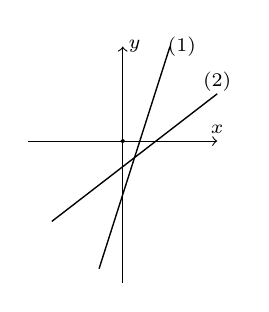
\begin{tikzpicture}[scale=0.6]
\tikzset {line01/.style={line width =0.5pt}}
\tikzset{line02/.style={line width =1pt}}
\tikzset{line03/.style={dashed,line width =0.9pt}}
\filldraw [black] (0,0) circle (1pt);
\draw [->] (-2,0) -- (2,0);
\draw [->] (0,-3) -- (0,2);
\draw[line01] (-1.5,-1.7) -- (2,1);
\draw[line01] (-0.5,-2.7) -- (1,2);
\draw (1.25,2) node {\scriptsize $(1)$};
\draw (2,1.25) node {\scriptsize $(2)$};
\draw (2,0.25) node {\scriptsize $x$};
\draw (0.25,2) node {\scriptsize $y$};
\end{tikzpicture}$ На рисунке изображены две прямые с уравнениями (1) $y_1=k_1x+b_1$ и (2)
$y_2=k_2x+b_2.$ Расставьте в порядке возрастания числа $k_1,\ k_2,\ b_1,\ b_2.$\\
